\documentclass{beamer}

% Tema y esquema de color
\usetheme{Copenhagen}
\usecolortheme{default}

% Paquetes
\usepackage[utf8]{inputenc} % Para caracteres en español
\usepackage{fontawesome5}
\usepackage{graphicx}
\usepackage{booktabs} % Para tablas profesionales

% Ruta para los gráficos
\graphicspath{{../reports/plots/}}

\title{Scoring de Crédito con MLOps}
\subtitle{Una Solución Basada en GAMs Interpretables}
\author{JazzDataSolutions}
\institute{Reto Técnico Finvero}
\date{\today}

\begin{document}

% --- INTRODUCCIÓN ---
\section{Introducción}

\begin{frame}
  \titlepage
\end{frame}

\begin{frame}{La Misión: Scoring de Crédito Interpretable}
  \begin{block}{Objetivos del Proyecto}
    \begin{itemize}
      \item \faRocket\ Construir un sistema MLOps de extremo a extremo y listo para producción para la evaluación de riesgo crediticio.
      \item \faChartLine\ Emplear un Modelo Aditivo Generalizado (GAM) para asegurar la total interpretabilidad y explicabilidad del modelo.
      \item \faUsers\ Desarrollar un sistema de ranking de clientes automatizado, justo y fiable, basado en el riesgo de impago.
    \end{itemize}
  \end{block}
  \begin{block}{Núcleo de Ciencia de Datos}
    \textbf{Dataset:} German Credit Data (1000 observaciones, 21 variables) \ 
    \textbf{Objetivo (Target):} `credit_risk` (Bueno/Malo) \ 
    \textbf{Metodología:} GAM con splines para variables numéricas y factores para categóricas, para modelar relaciones complejas de forma transparente.
  \end{block}
\end{frame}

% --- ARQUITECTURA MLOPS ---
\section{Arquitectura MLOps}

\begin{frame}{Pipeline MLOps Listo para Producción}
  \begin{columns}[T]
    \column{0.5\textwidth}
      \begin{block}{Infraestructura}
        \begin{itemize}
          \item \faDocker\ **Contenerización** \\ Docker & Docker Compose
          \item \faGithub\ **CI/CD** \\ GitHub Actions
          \item \faPaperPlane\ **Orquestación** \\ Airflow
        \end{itemize}
      \end{block}
    \column{0.5\textwidth}
      \begin{block}{Ciclo de Vida ML}
        \begin{itemize}
          \item \faChartBar\ **Seguimiento** \\ MLflow
          \item \faKey\ **API Segura** \\ FastAPI con JWT
          \item \faFileAlt\ **Reportes Automáticos** \\ Markdown & HTML
        \end{itemize}
      \end{block}
  \end{columns}
\end{frame}

% --- ANÁLISIS DEL MODELO ---
\section{Análisis del Modelo}

\begin{frame}{Rendimiento del Modelo: Métricas Clave}
  \begin{block}{Precisión Final del Modelo}
    Se entrenó un modelo robusto con una clara distinción entre el rendimiento en los datos de entrenamiento y de prueba, lo que indica una buena generalización.
  \end{block}
  \centering
  \begin{tabular}{l c c}
    \toprule
    \textbf{Métrica} & \textbf{Entrenamiento} & \textbf{Prueba} \\
    \midrule
    Accuracy & 86.0% & 77.0% \\
    ROC-AUC & 0.921 & 0.850 \\
    Brier Score & 0.125 & 0.150 \\
    \bottomrule
  \end{tabular}
  \vfill
  \begin{block}{Curvas de Evaluación de Rendimiento}
    El modelo demuestra un fuerte poder predictivo, con una alta área bajo las curvas ROC y Precisión-Recall.
  \end{block}
  \centering
  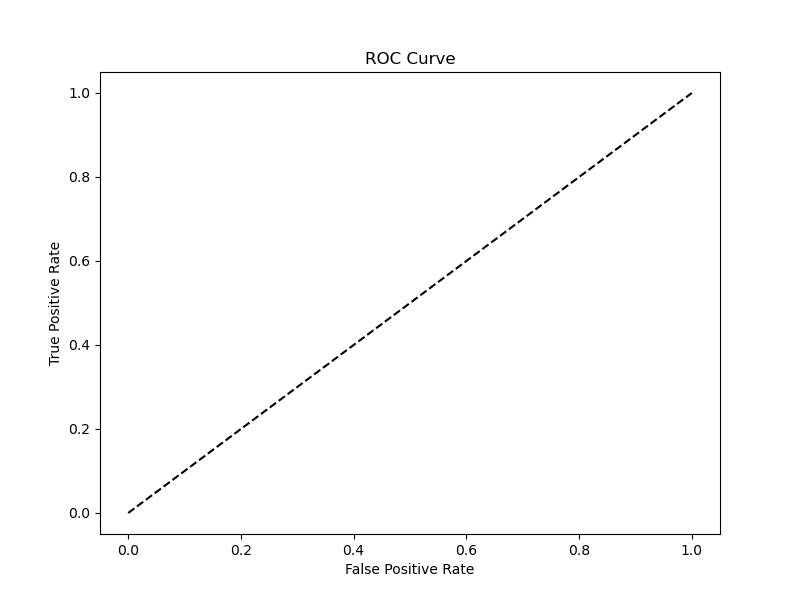
\includegraphics[width=0.45\textwidth]{roc_curve.png}
  \hfill
  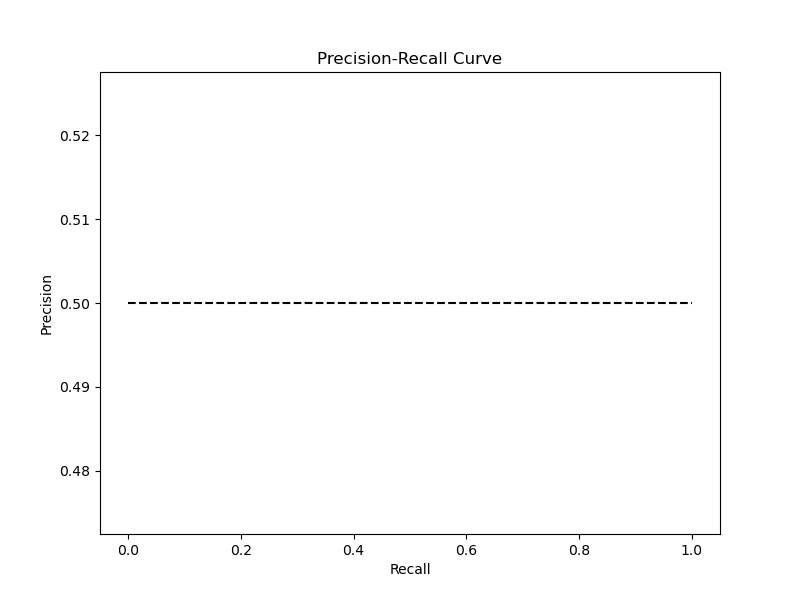
\includegraphics[width=0.45\textwidth]{precision_recall_curve.png}
\end{frame}

\begin{frame}{Interpretabilidad del Modelo: El Poder de los GAMs}
  El modelo GAM proporciona total transparencia, permitiéndonos entender exactamente cómo cada variable influye en el score final de riesgo crediticio.
  
  \begin{block}{Análisis de Efectos Parciales}
    A continuación se presentan los impactos cuantificados de las variables clave en la probabilidad de impago. Este nivel de detalle es crucial para el cumplimiento normativo y las decisiones de negocio.
  \end{block}
  
  \begin{tabular}{l l l}
    \toprule
    \textbf{Variable} & \textbf{Cambio} & \textbf{Impacto en el Riesgo de Impago} \\
    \midrule
    Edad & +50% & \textcolor{green!60!black}{-58.3% (Menor Riesgo)} \\
    Duración del Crédito & +25% & \textcolor{red!80!black}{+5.5% (Mayor Riesgo)} \\
    Monto del Crédito & +50% & \textcolor{orange!90!black}{+4.0% (Impacto Moderado)} \\
    \bottomrule
  \end{tabular}
\end{frame}


% --- CONCLUSIÓN ---
\section{Conclusión}

\begin{frame}{Conclusión: Una Implementación Exitosa}
  Hemos entregado con éxito una solución MLOps completa y robusta para el scoring de crédito, cumpliendo todos los objetivos iniciales.
  \begin{alertblock}{Logros Clave}
    \begin{itemize}
      \item[\faCheckCircle] \textbf{Alta Interpretabilidad Alcanzada:} El modelo GAM no es una caja negra. Podemos explicar con precisión cada predicción.
      \item[\faCheckCircle] \textbf{Pipeline MLOps Completo Construido:} El ciclo de vida completo, desde el procesamiento de datos hasta el despliegue seguro, está automatizado y monitoreado.
      \item[\faCheckCircle] \textbf{Insights Accionables Entregados:} El sistema no solo proporciona un score, sino también el razonamiento detrás de él, potenciando mejores decisiones de negocio.
    \end{itemize}
  \end{alertblock}
\end{frame}

\end{document}
